En un recipiente esférico de radio $16\,\mathrm{cm}$, la altura del agua medida desde el fondo es inicialmente $24\,\mathrm{cm}$ y a los $15$ días es $20\,\mathrm{cm}$. Suponga que el volumen evaporado por unidad de tiempo es proporcional al área de la superficie libre, con constante positiva y sin otras entradas ni salidas. Determine la altura en función del tiempo mientras queda agua. Puede usar $V(h)=\pi h^2(16-h/3)$.

\Needspace{7.32cm}
\begin{center}
\begin{minipage}{\linewidth}
\centering
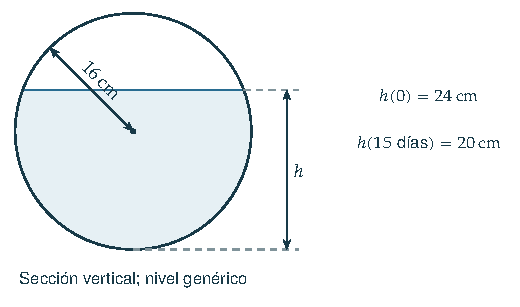
\includegraphics[width=9.86cm]{assets/M2-E0032-setup.pdf}\par
\smallskip{\small Sección del recipiente y referencia para medir la altura de agua.\par}
\end{minipage}
\end{center}
